\usetikzlibrary{petri, positioning}
\tikzset{every node/.style={node distance=2cm}}

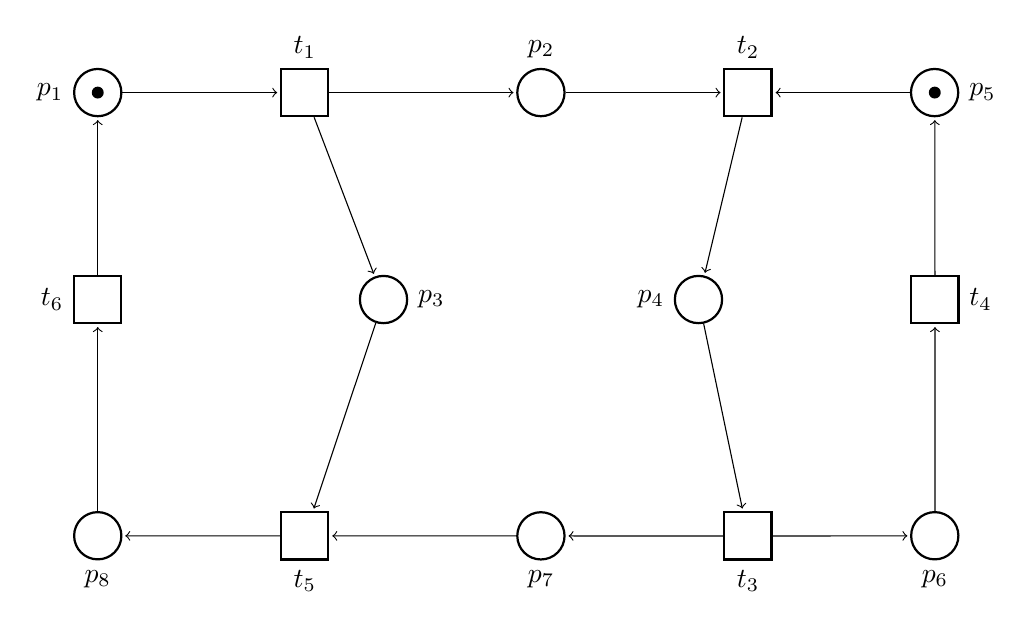
\begin{tikzpicture}[scale=1.2, every place/.style={minimum size=6mm, thick}, 
    every transition/.style={minimum size=6mm, thick}, bend angle=45]

    % Places
    \node[place, tokens=1] (p1) [label=left:$p_1$] {};
    \node[place] (p2) [right=of p1, xshift=3cm, label=above:$p_2$] {};
    \node[place] (p3) [below=of p2, xshift= -2cm,label=right:$p_3$] {};
    \node[place] (p4) [below=of p2, xshift= 2cm,label=left:$p_4$] {};
    \node[place, tokens=1] (p5) [right=of p1, xshift=8cm, label=right:$p_5$] {};
    \node[place] (p6) [below=of p5, yshift=-3cm,label=below:$p_6$] {};
    \node[place] (p8) [below=of p1, yshift=-3cm, label=below:$p_8$] {};
    \node[place] (p7) [right=of p8, xshift=3cm,label=below:$p_7$] {};
    

    % Transitions
    \node[transition] (t1) [right=of p1, label=above:$t_1$] {}
        edge[pre] (p1) 
        edge[post] (p3)
        edge[post] (p2);

    \node[transition] (t2) [right=of p2, label=above:$t_2$] {}
        edge[pre] (p2) 
        edge[pre] (p5)
        edge[post] (p4);

    \node[transition] (t3) [right=of p7, label=below:$t_3$] {}
        edge[pre] (p4) 
        edge[post] (p6)
        edge[post] (p7);

    \node[transition] (t4) [below=of p5, label=right:$t_4$] {}
        edge[pre] (p6) 
        edge[post] (p5);

    \node[transition] (t5) [right=of p8, label=below:$t_5$] {}
        edge[pre] (p7) 
        edge[pre] (p3) 
        edge[post] (p8);

    \node[transition] (t6) [below=of p1, label=left:$t_6$] {}
        edge[pre] (p8) 
        edge[post] (p1);
        
\end{tikzpicture}